\chapter{Background}
\label{chap:background}
Compared to ordinary galaxies, some have extraordinarily bright central regions, which can sometimes even outshine the host-galaxy emission by many orders of magnitude; these galaxies are called \textit{active galaxies} and their nuclei are referred to as \textit{active galactic nuclei} (AGN). The physical processes necessary to create such high luminosities ($L = 10^{43-48} \text{erg s}^{-1}$; e.g., \cite{Lusso2012AGNLuminosity}) within such a small volume were a subject of debate for years, but now are widely accepted to be connected to accretion onto the galaxies' central black holes (BHs; \cites{Salpeter1964AccretionTheory}{Zeldovich1964AccretionTheory}). These accreting objects have masses $M_{BH} \sim 10^{6-10} M_{\odot}$ (e.g., \cite{Peterson2004AstNach}) and an Eddington ratio exceeding $\lambda_{Edd}$\footnote{The ratio $L_/L_{Edd}$, where $L$ is the bolometric luminosity and $L_{Edd} = 1.5 \times 10^{38}M_{BH}/M_{\odot} \text{ erg s}^{-1}$ is the Eddington luminosity for a solar composition gas. This is the maximum isotropic luminosity a body can achieve while maintaining balance between radiation pressure and gravitational force.} $\approx 10^{-5}$. This threshold, chosen somewhat arbitrarily, excludes galactic nuclei with no significant accretion activity, such as that of the Milky Way, while still covering their full range of observed luminosities \parencite{Netzer2015AnnRev}. 

The \quotes{unified model} \parencites{Antonucci1993UnifiedAGN}{UrryPadovani1995UnifiedAGN} discussed in Section \ref{sec:UnifiedModel}, posits the black hole at the center of the AGN, surrounded by several distinct components, including an accretion disk, gas and dust clouds, and, in some cases, a relativistic jet (Figure \ref{fig:UnifiedAGNModel}). Each of these regions contributes emission into different wavelength regimes, resulting in these objects having detectable emission across the whole electromagnetic spectrum, as illustrated by the spectral energy distribution (SED) in Figure \ref{fig:AGNSED}. 

\begin{figure}[t]
    \centering
    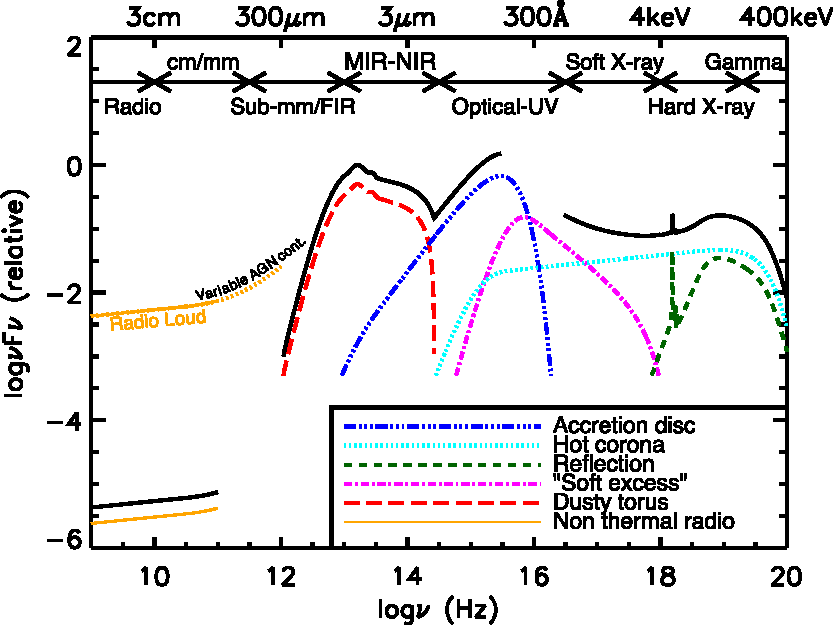
\includegraphics[height=0.7\textwidth]{assets/1_figures/SED-OG.pdf}
    \caption[AGN spectral energy distribution (SED) from radio frequencies to hard X-ray]{\label{fig:AGNSED} AGN SED from radio frequencies to hard X-ray, loosely based on the observed SEDs of radio-quiet quasars (e.g., \cite{Elvis1994QuasarSED}; \cite{Richards2006SEDCatalogues}). The black solid curve represents the total emission and the colored curves (shifted down for clarity) represent the individual constituents. The intrinsic shape of the SED in the mm-far infrared (FIR) regime is uncertain; however, it is credited to have a minimal contribution (to an overall galaxy SED) compared to star formation (SF), except in the most intrinsically luminous quasars and powerful jetted AGN. It should be noted that the relative contribution of each of the components can vary dramatically for different AGN types. Adapted from \textcite{Harrison2014PhDThesis}.}

\end{figure}

The gravitational energy released as the circumnuclear material falls inwards and loses angular momentum forms the accretion flow around the black hole, which acts as the primary source of AGN continuum emission. The disk gets heated up via viscous heating \parencite{Peterson1993RM}, producing a thermal spectrum that has a blackbody temperature peaking in the ultra violet (UV; $\approx 10-400$ nm) for a \quotes{typical} AGN (i.e., with $M_{BH} \approx 10^8 M_{\odot}$; $\lambda_{Edd} \approx0.1$); this is often referred to as the \quotes{big blue bump} (\cite{Harrison2014PhDThesis}; Figure \ref{fig:AGNSED})

The thermal disk photons, also called \textit{seed photons}, are Comptonized by highly energetic electrons that are located at the \textit{corona} (\S \ref{ssec:Corona}) to form the X-ray power-law spectrum observed in Figure \ref{fig:AGNSED}. These high energy photons can also reflect off the accretion disk and/or the \textit{torus} (\S \ref{ssec:Torus}), producing the additional hard X-ray \quotes{reflection} component. In a majority of AGN X-ray spectra, there is an additional \quotes{soft excess} \parencites{Singh1985SE}{Arnaud1985SE} at energies less than $\sim 2$ keV. This emission is above what would be expected from simple accretion disk models and its origin is still a topic of discussion. Two proposed models (which could be simultaneously true) to explain this soft excess are: relativistically blurred ionized reflection from the inner accretion disc (e.g., \cite{Crummy2006BlurredReflectionSE}), or Comptonization in a \quotes{warm corona} located near the surface of the accretion flow (e.g., \cite{Ballantyne2022WarmComptSE}).  


% In the ionized reflection model, soft excess arises from blurred ionized reflection, where fluorescent lines from reprocessed X-ray emission are smeared due to the strong gravitational field near the SMBH (e.g., Ross & Fabian 2005; Garc´ıa & Kallman 2010; Dauser et al. 2016; Ding et al. 2024). 

%In contrast, the warm corona model attributes the SE to thermal Comptonization of seed photons from the AD in an optically thick, warm plasma (e.g., Magdziarz et al. 1998; Petrucci et al. 2018), which is distinct from the hot corona

The infrared (IR; $\approx 1-1000$ $\mu$m) band, is mostly sensitive to the reprocessed emission of the accretion disk by the torus. Although the shape of this IR emission varies from source to source, the peak of this dusty component is usually around $\lambda \approx 20-50$ $\mu$m and falls steeply at longer wavelengths \parencite{Harrison2014PhDThesis}. In the sub-mm/far-infrared (FIR), or sometimes even in the mid-infrared (MIR), stellar heated emission from cooler dust dominates over AGN heated emission \parencite{Lutz2014SFRDust}. 

AGN cover a wide range of radio luminosities, which can differ by several orders of magnitude between radio-quiet (RQ) and radio-loud (RL) sources, now more aptly referred to as non-jetted and jetted, respectively \footnote{While RL/RQ has been the historical terminology, radio-quiet sources are not truly radio-silent but rather \quotes{radio-faint} and they are, however, $\gamma$-ray quiet \parencite{Padovani2017Onthe2mainclasses}.} (orange lines in Figure \ref{fig:AGNSED}). The latter type makes up only a minority of the AGN population (e.g., \cite{Padovani2011Non-JettedAGNPop}) with objects that present highly collimated, relativistic radio \textit{jets} (\S \ref{ssec:Jets}) and extended radio structures such as lobes and hotspots, that together emit strong non-thermal radiation and, occasionally, a $\gamma$-ray jet. On the other hand, the spectrum of non-jetted objects is dominated by thermal emission in most bands and the origin of their radio emission has not been clearly established. Some possibilities include coronal activity or synchrotron radiation from particles accelerated in shocks (see e.g., \cite{Laor2008RQEmission}; \cite{Ishibashi2011RadioQuietAGN}).

% \footnote{While non-jetted AGN are actually not radio-quiet but \quotes{radio faint}, they are $\gamma$-ray-quiet \parencite{Padovani2017Onthe2mainclasses}.}
% bimodality in radio-loudness dist

\section{Unified Model of AGN}
\label{sec:UnifiedModel}

Because different wavebands probe different physical elements, AGN selected at particular wavelengths often exhibit distinct properties, leading to a rich phenomenological classification (Figure \ref{fig:AGNspectra}). Reality, however, is much simpler because now we know that most of these classes differ from each other only by a small number of parameters, such as: orientation, accretion rate, the presence of jets, and possibly the host galaxy and environment (see \textcite{Padovani2017whatisaname} and references there-in). This suggests that the numerous brands do not necessarily correspond to fundamentally different physical objects, but instead motivate a unifying framework capable of explaining their apparent diversity.

\begin{figure}[t]
    \centering
    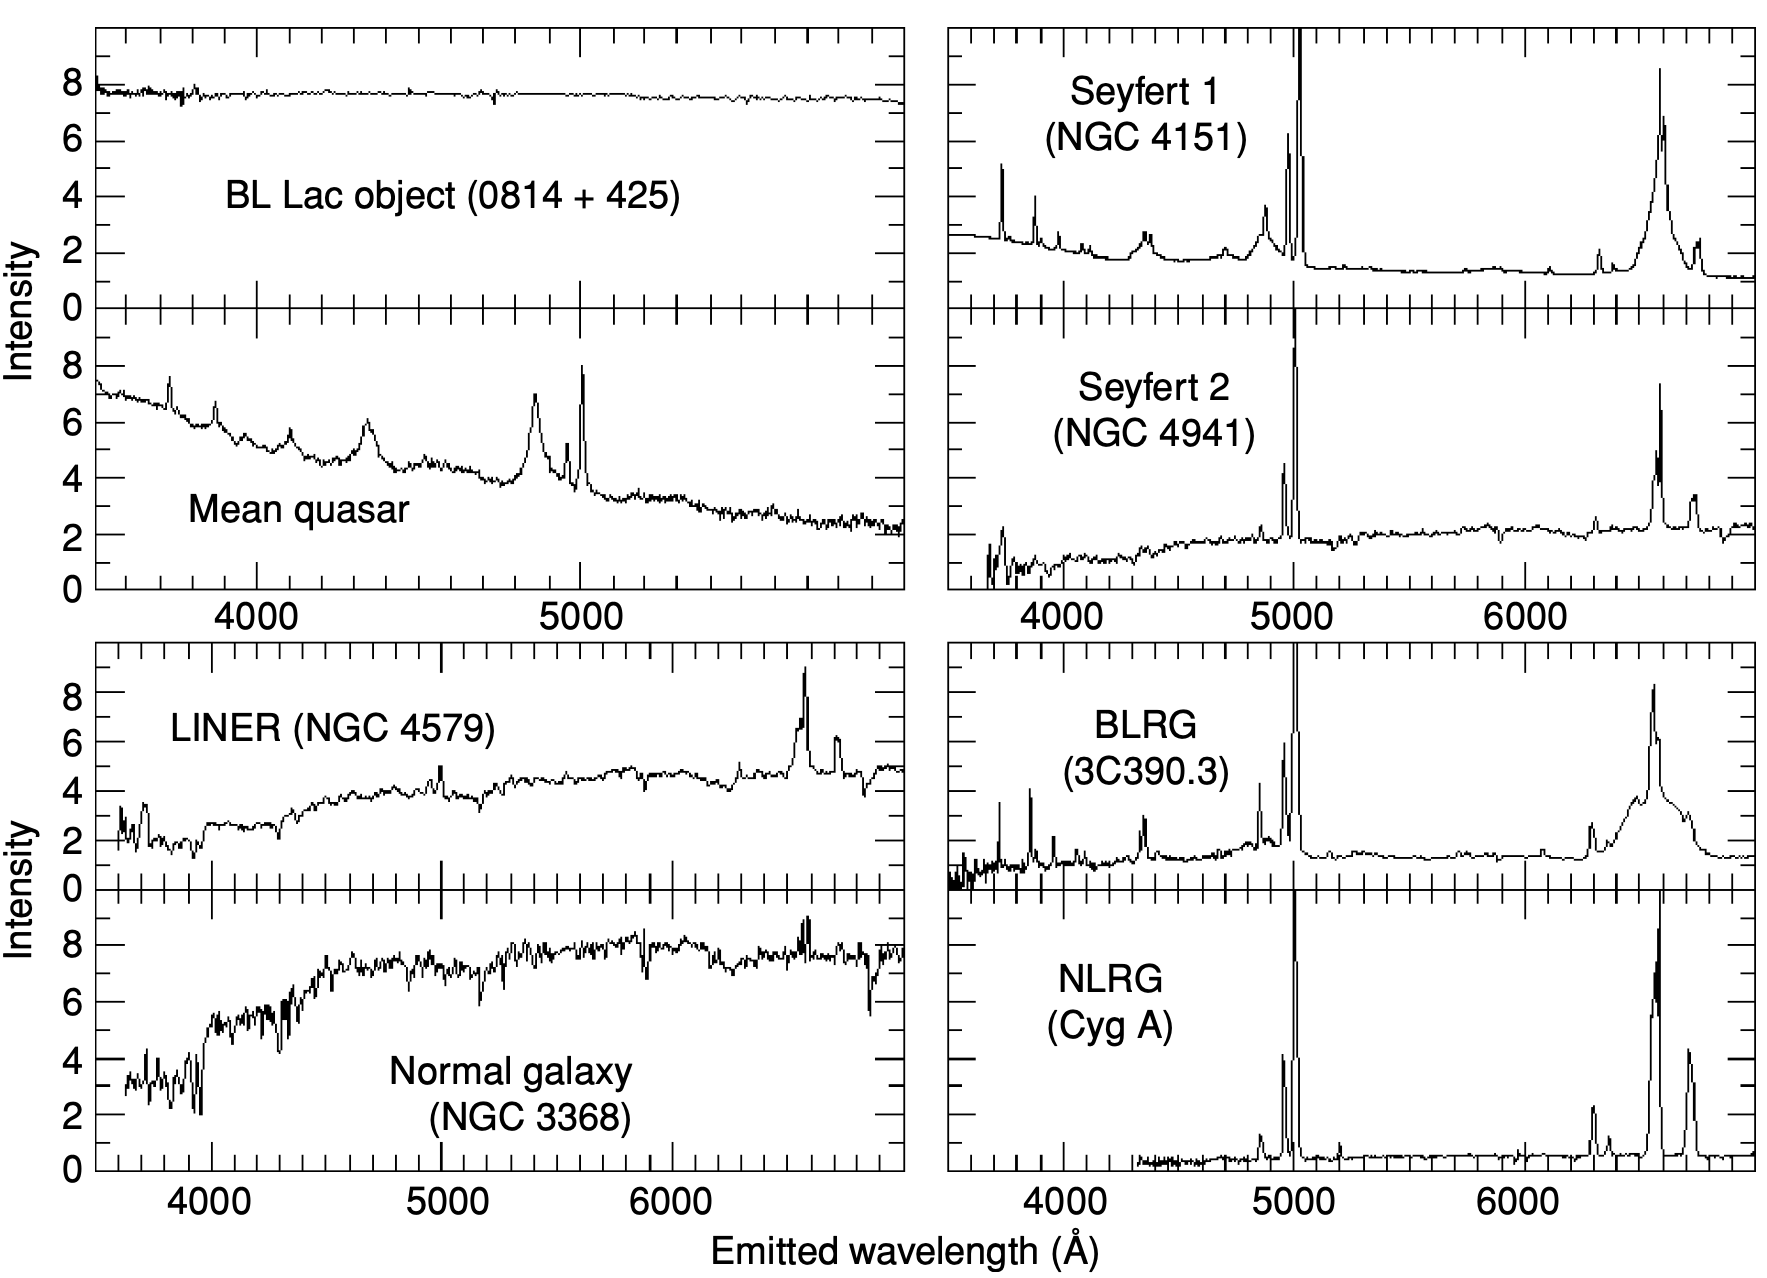
\includegraphics[height=0.70\textwidth]{assets/1_figures/AGN-Spectra.png}
    \caption[Typical optical spectra of different AGN classes]{\label{fig:AGNspectra} Optical spectra of representative AGN classes, from the (essentially featureless) BL Lac objects (Top left) through the radio galaxies and QSOs \parencite{SewardCharles1995ExploringtheXrayUniverse}. Note the presence of both broad and narrow emission lines in quasars, Seyfert 1 galaxies and broad-line radio galaxies (BLRG), while Seyfert 2 galaxies, low-ionisation nuclear emission region (LINER) galaxies and narrow-line radio galaxies (NLRG) only show narrow permitted and forbidden lines. A normal galaxy spectrum (Bottom left) is shown for comparison.}
\end{figure}


This unification idea arose shortly after the discovery of \textit{quasars} (QSOs\footnote{The term quasar historically stands for “quasi-stellar radio source”; throughout this thesis it is used more broadly to refer to very luminous AGN.}), when the observed variety of AGN prompted questions about the role of the observer's orientation relative to the AGN axis. \textcite{Blandford1978BlLacConference} proposed that BL Lac objects were radio galaxies viewed down the axis of a relativistic jet, where \textit{relativistic beaming} (\S \ref{ssec:Jets}) would cause the non-thermal continuum to appear very bright and the emission lines weak in comparison. The same object, viewed from the side, would have normal emission-line equivalent widths, and the radio structure would be dominated by the extended lobes rather than the core \parencite{Shields2004NED}.  
% \cite{Seyfert1943Emission}?? Seyfert 1 galaxies are characterized by the presence of broad optical permitted lines (FWHM>1000 km/s), such as Hα and Hβ, that are not observed in Seyfert 2 galaxies However, the presence of both strong high ionization and low ionization narrow (FWHM<1000 km/s) forbidden lines (such as [O iii], [Ne iii], [O ii], [O i], [N ii], [S ii]), and several very high ionization coronal lines (such as [Fe x], [Fe xi], [Si ix], [Si x]) is common to both types of Seyfert galaxies and with similar line ratios. The latter finding suggested that all Seyfert galaxies are powered by the same intrinsic engine.

Further evidence came from spectropolarimetry, the measurement of the polarization state of the incoming light from a source as a function of wavelength. Seyfert galaxies \parencite{Seyfert1943Emission} are primarily divided into two types based on their optical spectra: Type 1 objects exhibit both broad permitted emission lines such as H$\alpha$ and H$\beta$ (FWHM $> 1000$ km s$^{-1}$) and narrow forbidden lines such as [O III] and [Ne III] (FWHM $< 1000$ km s$^{-1}$), while Type 2 objects show only the narrow component. Crucially, both types share the same high- and low-ionization narrow forbidden lines with similar line ratios, suggesting they are powered by the same intrinsic engine.

\begin{figure}[t]
    \centering
    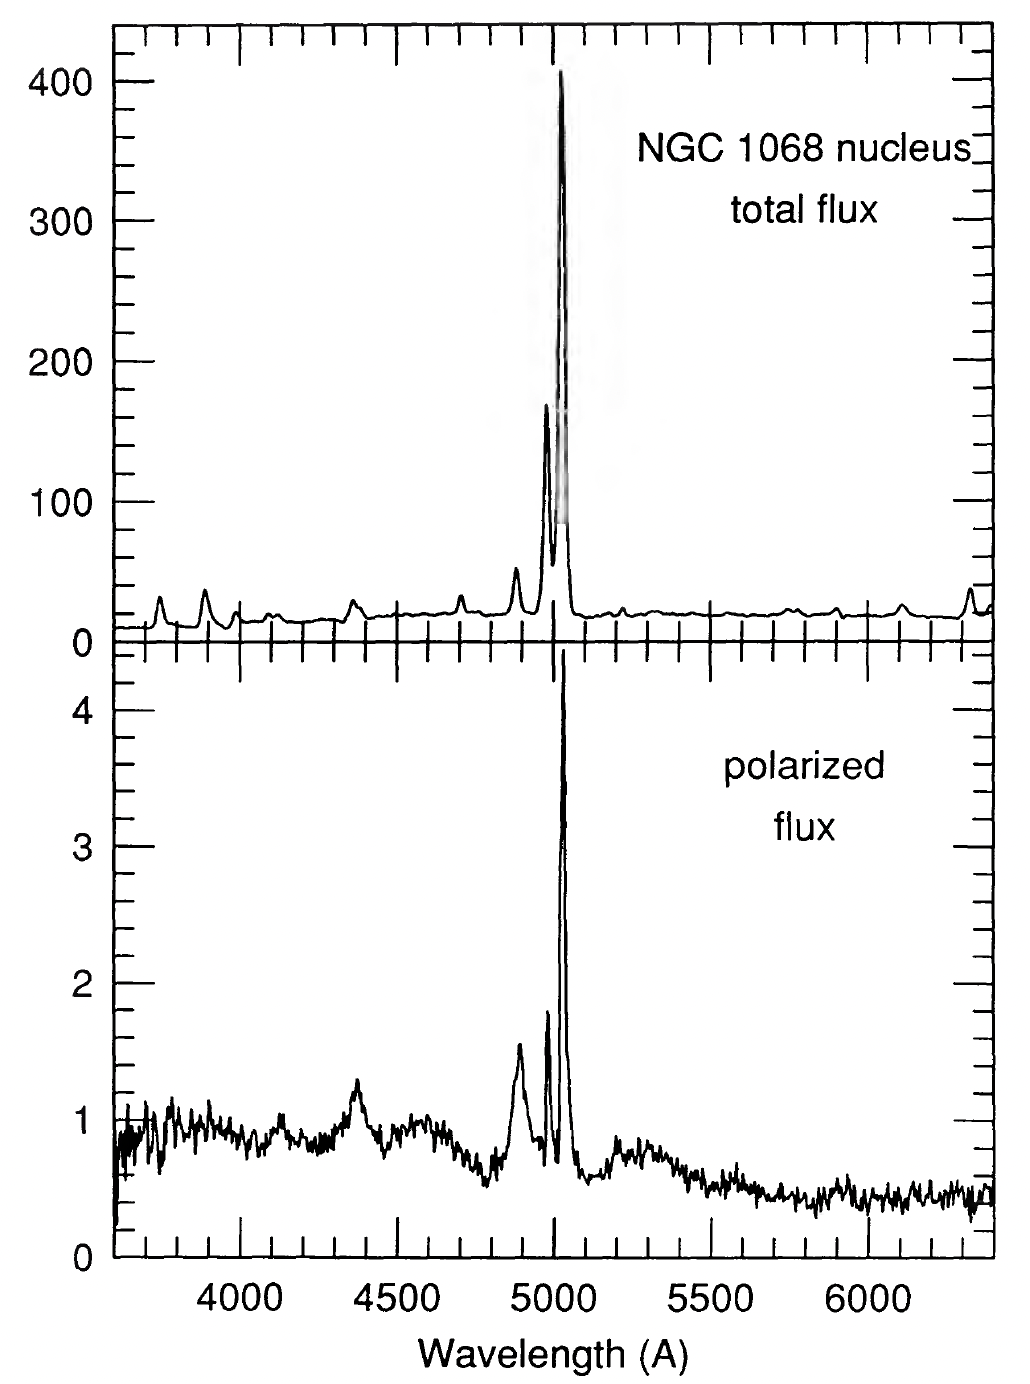
\includegraphics[height=0.7\textwidth]{assets/1_figures/NGC1068.png}
    \caption[NGC 1068 spectropolarimetry revealing the hidden broad line region (BLR)]{\label{fig:NGC1068} Optical spectra of the nucleus of NGC 1068 \parencite{Miller1991NGC1068}. The total spectrum (Top) shows the narrow emission lines expected for Type 2 AGN, while the polarized flux spectrum (Bottom) reveals the broad permitted emission lines characteristic of unobscured Type 1 AGN.}
\end{figure}

\textcite{AntonucciMiller1985SpecPolarimNGC1068} confirmed this by analyzing the polarized flux of NGC 1068, a Seyfert 2 galaxy\footnote{It should be noted that a subset of Type 2 AGN ($\sim 30\%$), sometimes referred to as \quotes{true Type 2} objects, show no detectable broad lines even in polarized light and little X-ray absorption (see \cite{Netzer2015AnnRev} and references there-in).}, resembled that of a Seyfert 1 spectrum, as can be seen in Figure \ref{fig:NGC1068}. This was interpreted as the broad-line region (BLR; \S \ref{ssec:BLR}) and the central continuum source being blocked from direct view by a dusty torus, while free electrons above the nucleus scatter a fraction of the nuclear light towards the observer, polarizing it in the process. The broad lines had gone unnoticed in direct light because this scattered component was too faint relative to the strong narrow-line emission from the narrow-line region (NLR; \S \ref{ssec:NLR}), which extends beyond the obscuring torus and is therefore visible regardless of orientation. 


\begin{figure}[t]
    \centering
    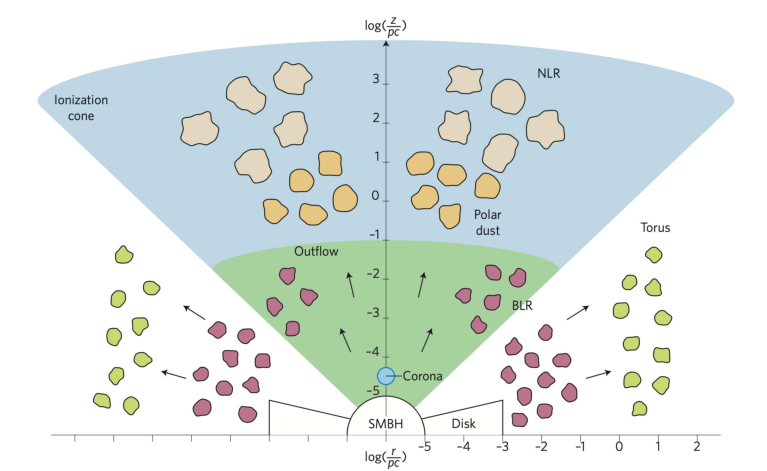
\includegraphics[height=0.55\textwidth]{assets/1_figures/UnifiedAGNModel.pdf}
    \caption[Schematic view of the the innermost regions of (non-jetted) AGN]{\label{fig:UnifiedAGNModel} Overview of the innermost regions around a non-jetted accreating supermassive black hole (SMBH). Typical scales along the polar and equatorial directions (for nearby AGN) are shown. Different colors depict regions with different densities or compositions. Taken from \cite{RamosAlmeida2017AGNNuclearObscuration}.}
\end{figure}

Multiple efforts such as those recounted above (e.g., \cites{Antonucci1984SpecPolarimOtherGalax}{OrrBrowne1982AGNBeaming}) were fundamental to the development of the \quotes{favoured} unified model of AGN introduced in this section. Whilst it has been succesful in homogenizing many kinds of active nuclei, recent works point to the conclusion that a picture based primarily on orientation and obscuring material is incomplete (e.g., \cite{Bianchi2012UMAGNcons}). Nonetheless, the major aspects of the model are sufficient for the purposes of this thesis; in the sections below, the primary components are explained briefly, while additional features such as polar dust and large-scale outflows (also visible in Figure \ref{fig:UnifiedAGNModel}) are discussed shortly when relevant but are not treated as separate subsections.
%AGN structure, from the very center to host-galaxy scales, is mainly constituted by: a massive central BH, an X-ray corona, an accretion disk, a broad-line region, a torus, and a narrow-line region (Figure \ref{fig:UnifiedAGNModel}), with radio-loud AGN also hosting relativistic jets. Additional features such as polar dust and large-scale outflows (also visible in Figure~\ref{fig:UnifiedAGNModel}) are discussed briefly in the context of the relevant components but are not treated as separate subsections here.

\subsection{Accretion Disk}
\label{ssec:AccretionDisk}

%by “optically thick", we here mean media optically thick to the photoionization continuum 
The standard framework of the optically thick, geometrically thin accretion disk \parencite{ShakuraSunyaev1973BHAppearance} described above applies to SMBHs with moderate to high Eddington ratios ($10^{-2} \lessapprox \lambda_{Edd} \lessapprox 1$; \cite{Ricci2026unificationmodelsactivegalactic}), where the accretion flow is considered radiatively efficient. This scheme describes the disk as a composition of Keplerian rings, nested and coupled to each other by viscous forces, likely driven by turbulence and magnetic instabilities, the magneto-rotational instability (MRI; \cite{Balbus1998TurbulenceAccretionD}) being the most widely quoted. The outer, slower ring brakes the inner faster one, transporting the angular momentum outwards and allowing material to spiral inward. Friction between the rings produces heat that is dissipated as blackbody emission with a characteristic maximum temperature of $T \sim 10^5$ K for the \quotes{typical} AGN described above \parencite{Netzer2013PhyEvolofAGNBook}, yielding the multi-temperature spectrum depicted in Figure \ref{fig:AGNSED}. The continuum emission of the accretion disk varies with time depending on the dynamics of the infalling matter (see Chapter \ref{chap:variability}).

% the disk can be divided into 3 regions depending on R that determine the as density profile: 
% the OUTER REGION at large r, in which P_gas > P_rad and the opacity is controled by free-free absorption. 
% the MIDDLE REGION, at smaller R, in which P_gas < P_rad but opacity is mainly due to electron scattering and
% the INNER REGION, at very small R, where P_rad > P_gas but still scattering dominates the absorption opacity
% The fact that quasars become bluer as they brighten is consistent with a thermal origin (e.g., Giveon et al. 1999; Trevese et al. ` 2001; Geha et al. 2003).Moreover, the thermal timescale is sensitive to the disk viscosity.


% viscosity is supposed to be prop to pressure

% within the standard model, the disk's inner regions are expected to be dominated by radiation pressure, and therefore both thermanly and viscously unstable. Magnetically supported models dont have this instabilities (eg Begelman & Pringle 2007) (net cooling fct: T vs radiation/P_{gas}, has an S-shape that allows coexistence of gas at different pressures and temperatures for the same pressure ratio i.e. for a given ratio we have 3 solutions, unstable, hot or cold) (Gonçalves 2006). We expect (exponentially growing) thermal instabilities on timescales sim to the thermal timescale (which for AGN is months/years) but there is no evidence for such in lightcurves spanning \gtrsim t_{th} 

%Alternatively, if part of the accretion energy is dissipated in a hot corona, then there is no longer any runaway heating in the disk, as additional cooling is provided by the corona (Svensson & Zdziarski 1994).

Most QSOs in the local universe are thought to accrete through thin disks, yet contrasting accretion scenarios are possible depending on the Eddington ratio (Figure \ref{fig:EddRatioDist}). At $\lambda_{Edd} \lesssim 10^{-2}$, the disk becomes optically thin and with an Advection Dominated Accretion Flow (ADAF, \cite{Narayan1994ADAF}), radiating weakly and with minimal optical/UV emission. Conversely, at $\lambda_{Edd} \gtrsim 1$, theoretical works have predicted that the SMBHs accrete rapidly through \quotes{slim} (or \quotes{thick}) disks, showing very different SEDs than their slower counterparts and powerful outflows (e.g., \cite{Kubota2018AGNSEDHighEddR}; \cite{Giustini2019AGNOutflowsHighEddR}).

\begin{figure}[t]
    \centering
    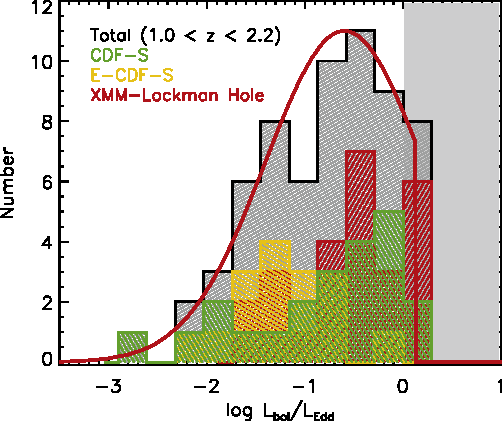
\includegraphics[height=0.45\textwidth]{assets/1_figures/EddRatioDist.pdf}
    \caption[Eddington ratio distribution of broad-line AGN at $1.0 < z < 2.2$.]{\label{fig:EddRatioDist} Eddington ratio distribution of broad-line AGNs at $1.0 < z < 2.2$. Different X-ray surveys are represented as different color histograms, and the black histogram pictures all the combined distributions. The gray shade illustrates the Eddington limit ($\lambda_{Edd} = 1$) and the red solid line corresponds to a log-normal fit with a peak of log $L/L_{Edd} = -0.6$ \parencite{Suh2015EddRatioDist}.}
\end{figure}


\subsection{Corona}
\label{ssec:Corona}

Numerical simulations of magnetohydrodynamical accretion disks have shown that the dissipation of the magnetic energy built up by the MRI naturally produces a hot, active corona located within a few gravitational radii ($R_g = G M/c^2$) of the accretion disk \parencites{Balbus1998TurbulenceAccretionD}{Miller2000MagnetoCorona}{Fabian2009Corona}. This compact region of ionized gas reaches temperatures of $T \sim 10^9$ K \parencite{Kara2025SMBHXRayReview}, and its rapid variability (see Chapter \ref{chap:variability}) is consistent with such a small emitting region. The corona contributes approximately 5\% of the AGN bolometric output \parencite{Ricci2026unificationmodelsactivegalactic}, a fraction that decreases with increasing $\lambda_{Edd}$, with lower $\lambda_{Edd}$ systems showing stronger X-ray emission relative to the disk \parencite{Padovani2017whatisaname}.

% the corona is optically think tau \sim 1-3

% The relative strength of the power-law component with respect to the quasi-blackbody one, due to thermal emission from an accretion disc, is used to classify the different observed spectra from different sources into two main states: the hard one (when the power-law component dominates) and the soft one (when, on the contrary, the disk blackbody component is prominent). (Marloni 2001)
\subsection{Broad-line Region}
\label{ssec:BLR}

The broad-line region consists of high density gas clouds ($\gtrsim 10^{9}$ cm$^{-3}$) predominantly in Keplerian motion at luminosity-dependent distances of $0.01-1$ pc from the central black hole \parencite{Netzer2015AnnRev}, well within the \textit{dust sublimation radius} (see \S \ref{ssec:Torus}). The BLR is therefore dust free, emitting broad permitted and semi-forbidden emission lines with velocity widths ranging from $1,000$ to $20,000$ km s$^{-1}$ \parencite{Ricci2026unificationmodelsactivegalactic}, wideness caused by \textit{Doppler broadening}\footnote{Doppler broadening refers to the superposition of emission from clouds moving at different directions/velocities along the line of sight produces a single broadened line whose width reflects the velocity dispersion of the gas.}. Ionizing photons from the accretion disk and corona illuminate these clouds, which subsequently exhibit ionization stratification with respect to radius, with higher ionization species located closer to the central source \parencite{Netzer2013PhyEvolofAGNBook}. The physical origin of the BLR remains an open question, some of the models presented in the literature include radiation pressure driven disk winds \parencite{Murray1995DiskWindBLR} and failed dust-driven wind from the disk surface (Figure \ref{fig:CzernyBLR}; \cite{Czerny2011WindOriginBLR}). 
Notably, the distance of the BLR from the central source scales with the AGN luminosity as $R_\mathrm{BLR} \propto L^{1/2}$ \parencite{Kaspi2000BLRSScalingL}, a relationship that is fundamental in reverberation mapping studies (\S \ref{ssec:RebMap}).

% Dimitrijevic: 
% chemi-ionazation (including processes of associative ionization) and the corresponding recombination processes. Atom-rydberg atom chemi-ionization/Recombination processes in the hydrogen clouds in BLR in AGN
%The role of collisional processes 
% the influence of collisional ionization proceses 
% VAMDC: Virtual Atomic and Molecular Data Center, CHIANTI, NIST, VALD

\begin{figure}[t]
    \centering
    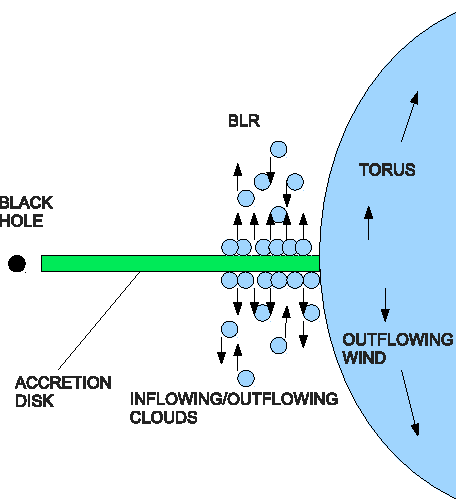
\includegraphics[height=0.58\textwidth]{assets/1_figures/BLR.pdf}
    \caption[Schematic of the BLR formation via a failed disk wind]{\label{fig:CzernyBLR} Schematic of the BLR geometry and its location relative to the accretion disk and dusty torus. The figure also illustrates the failed wind scenario of \textcite{Czerny2011WindOriginBLR}: dust forms in the atmosphere of the inner accretion disk at radii where $T_{eff} < T_{sub}$, is launched as a wind, but then is suppressed by the radiation from the central source and partially falls back, giving rise to the inflowing and outflowing clouds that make up the BLR.}
\end{figure}

\subsection{Dusty Torus}
\label{ssec:Torus}
As posed previously, the presence of an assymetric \quotes{dusty obscurer} has successfully unified apparently different AGN classes. When observed edge-on (i.e., at high inclination angles), this torus\footnote{For convenience, we keep referring to this obscuring matter as the torus despite the fact that it could have a different (and more complex) geometrical distribution (e.g., \cites{Nenkova2008ClumpyTorus}{Stalevski2012TwoMediumTorus}).} obscures the innermost regions of the AGN and hides the broad emission lines; conversely, when viewed face-on (at lower inclination angles), there is a clear line of sight to the BLR and accretion disk (Seyfert 1 vs Seyfert 2 in Figure \ref{fig:AGNspectra}). This structure is conceptualized as an optically thick structure surrounding the central engine at scales larger than that of the BLR and luminosity dependent dimensions ranging from $0.1-10$ pc \parencite{Netzer2015AnnRev}. Its inner boundary coincides is the dust sublimation radius ($R_\mathrm{sub}$), beyond which the dust can survive the radiation from the central engine. This radius corresponds to the distance at which the dust temperature reaches the sublimation threshold ($T_{sub} \sim 1400-1800$ K for silicate and graphite grains respectively; e.g., \cites{Barvainis1987DustSublimation}{Netzer2015AnnRev}). 

In addition to being responsible for the IR reprocessed emission on the AGN SED (Figure \ref{fig:AGNSED}), the torus acts as a gas and dust reservoir that regulates the material available for accretion onto the black hole. Its geometry, believed to contain a central opening, also collimates the AGN radiation into bi-conical ionization cones along the polar direction \parencite{Pogge1988IonizationCones}, which illuminate the NLR (\S \ref{ssec:NLR}). Furthermore, AGN drive large scale winds and outflows along these directions, powered by radiation and magnetic pressure from the central engine, which can interact with and regulate the host galaxy interstellar medium \parencite{Ricci2026unificationmodelsactivegalactic}. 

\subsection{Relativistic Jets}
\label{ssec:Jets}
Jets are thought to be powered by the extraction of rotational energy from the SMBH via strong electromagnetic fields \parencite{Blandford1977JetMechanism}, and can extend to Mpc scales from their host galaxy (Figure \ref{fig:ClarkeGRG}; \cite{Clarke2017GiantJettedGalaxy}). 

\begin{figure}[t]
    \centering
    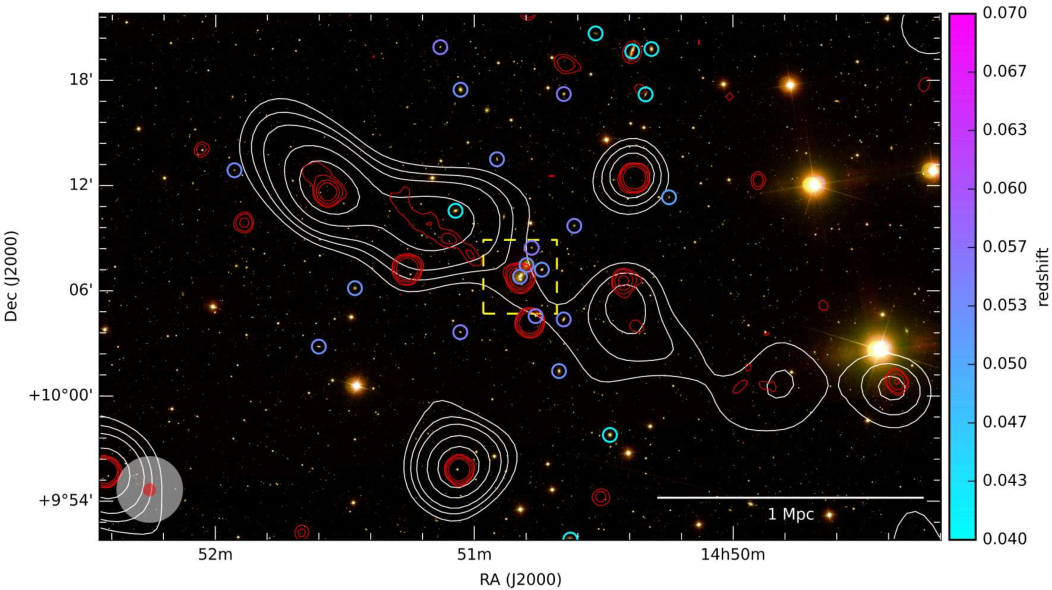
\includegraphics[width=\textwidth]{assets/1_figures/GRG.pdf}
    \caption[Radio contours of a giant radio galaxy extending to Mpc scales]{\label{fig:ClarkeGRG} SDSS optical image (composite from bands $g$, $r$ and $i$) of the galaxy group UGC 9555 overlaid with NVSS contours (red) and LOFAR MSSS radio contours (white) revealing the size of the giant radio galaxy (GRG). The white bar indicates a physical scale of 1 Mpc, illustrating how AGN jets can extend well beyond the boundaries of their host galaxies. Adapted from \cite{Clarke2017GiantJettedGalaxy}.}
\end{figure}

Their launch point coincides with the location of the corona, in the immediate vicinity of the accreting object, and their apparent velocities range from mildly to highly relativistic motion. The broadband emission of jets is characterised by a double-peaked SED: the low-energy peak, spanning radio to optical wavelengths, arises from synchrotron radiation of relativistic electrons spiralling in the jet magnetic field, while the high-energy peak, from X-ray to $\gamma$-ray energies, is thought to result from inverse-Compton scattering of soft photons from the BLR and accretion disk by the same relativistic electrons \parencite{Netzer2013PhyEvolofAGNBook}. %check screenshot from the presentation 

% Low/Intermediate/High Sinchroton Peak (the first peak of the SED), most are LSPs

Their observed properties depend strongly on orientation because relativistic beaming could make an approaching jet appear significantly brighter than a receding one. This effect, known as \textit{Doppler boosting}, arises when the jet plasma has bulk relativistic motion that concentrates the emitted radiation into a narrow cone in the direction of motion, amplifying the observed flux and variability for jets viewed close to face-on and explainig the extreme characteristics observed on blazars \parencite{UrryPadovani1995UnifiedAGN}. Jets are also thought to play a role in galaxy evolution by injecting energy into the surrounding environment, a process referred to as radio-mode feedback \parencite{Fabian2012AGNFeedback}.
% blazars are AGNs with relativistic jet oriented close to our line of sight, the observed flux is doppler boosted and variability is fastened (by the same Doppler factor? \delta = 15). Both FSRQs (can be only LSP) and BL Lacs (can be LSP, ISP or HSP) are RL, jet dominated AGN.
% synchroton self-absorption decreases steeply with frequency


\subsection{Narrow-line Region}
\label{ssec:NLR}
This assymetric region is extended enough to be resolved optically (e.g., \cite{Fischer2013NLRobs}; \cite{Polack2024NLRobsHST}), spanning hundreds or even thousands parsecs along the ionization cones (Figure \ref{fig:UnifiedAGNModel}). The NLR, just as the BLR, is photoionized by the central engine and exhibits optical emission lines, kinematically broadened with typical widths of $10^{2-3}$ km s$^{-1}$ \parencite{Bennert2005}, with most lines falling within the $350-500$ km s$^{-1}$ range \parencite{Ricci2026unificationmodelsactivegalactic}. 
\begin{figure}[t]
    \centering
    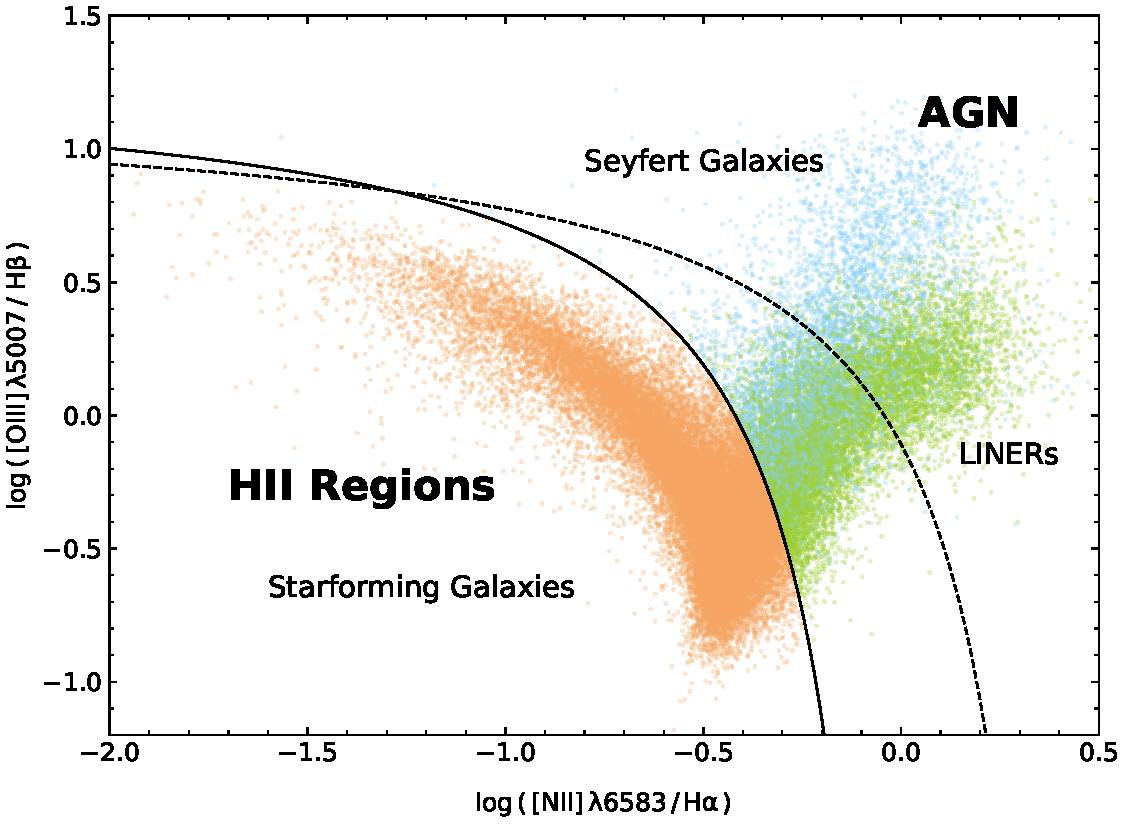
\includegraphics[width=0.85\textwidth]{assets/1_figures/bpt_alternative.pdf}
    \caption[SDSS galaxies in the classical BPT diagram.]{\label{fig:BPT} Select galaxy objects from the Sloan Digital Sky Survey (SDSS) catalog shown in the BPT diagram. It plots the intensity of the [OIII] $\lambda5007$ forbidden transition relative to that of the H$\beta$ line versus the ratio of [NII] $\lambda6583$ to H$\alpha$ on logarithmic axes. Using this to infer ionization states and abundances of the emitting medium enables us to reconstruct the origin of the dominant radiation in the galactic host, which has led to various approaches for the classification of these objects. Depicted is the theoretical delimiter by \textcite{Kewley2001StarburstModel} as well as the empirical line by \textcite{Kauffmann2003AGNBPT} to distinguish predominantly starforming galaxies from AGN. Additionally, the \textcite{Schawinski2007BPT} boundary sorts AGN into efficiently accreting Seyfert and inefficient LINER subtypes. Courtesy of Fritz A. Agildere.}
\end{figure}

Compared to the BLR, the NLR has a lower electron density ($\sim 10^{2-3}$ cm$^{-3}$), allowing forbidden transitions to occur without being collisionally suppressed. The presence of these forbidden lines, together with the high ionization state of the gas, can trace AGN activity and makes the NLR emission diagnostically distinct from that of star-forming regions, a separation commonly visualised using emission line ratio diagrams such as the Baldwin-Phillips-Terlevich (BPT) diagram \parencite{Baldwin1981BPT} (Figure \ref{fig:BPT}). 
